\subsection{Idle Experiment}

During the experiment from \cref{sec:experiment_one}, it was observed that the idle experiments were significantly lower than the expectations from \cref{subsec:expec_energy_consumption}. Because of this some further investigation into the results was conducted. This was true for all of the software based measuring methods as can be seen in \cref{fig:TestCaseIdle_Cores_comparison_energy_without_outliers_avg_watts}, here the low measurements for the idle case for the software measurements can be seen.
The hardware measurements was within the lower range of the expectations, the idle case for the hardware measurements can be seen in \cref{fig:TestCaseIdle_Cores_comparison_energy_without_outliers_avg_watts}, where the energy of the whole DUT can be seen in the idle test case.Initially we expected some erroneous implementation of the idle test case. 


            \begin{figure}
                \centering
                \begin{tikzpicture}
                    \pgfplotsset{%
                        width=1\textwidth,
                        height=0.5\textheight
                    }
                    \begin{axis}[
                        xlabel={Start temperature},
                        ylabel={Average dynamic energy (watt)},
                    ]
                    
                    \end{axis}
                \end{tikzpicture} 
            \caption{A graph illustrating the energy consumption of Cores for test case TestCaseIdle with regards to the temperature of the DUT} \label{fig:TestCaseIdle_Cores}
            \end{figure}
            

The original idle test case, was implemented using \texttt{Thread.Sleep()}, so we tried replacing this part of the test case with \texttt{Task.Delay()} to see if this had an impact. The results from this was identical to the previous results, so we ruled out problems with the testCase itself. The next step was looking into P-states and C-states on the CPU\cite[]{PCStat}, where the P-states are performance states which provides a way to change the frequency and voltage of the CPU. P0 would be max performance and higher values of P underclocks the CPU. The C-states become relevant when the CPU is doing little to no work, as they turn off certain parts of the CPU to drastically reduce power consumption. Since the problem only seemed to occur during the idle experiments we suspected it had something to do with the C-states. To test whether the C-states were causing the low energy consumption or not we tried to disable them in the BIOS. This was however only possible on the workstation as the Surface devices had very limited options available. Running the experiments again with the C-states disable seemed to have little to no effect of the measurements. Looking more into the BIOS we discovered that the TUF B360M-PLUS GAMING motherboard had three modes, performance mode, Max power saving mode and automatic. Max power and performance mode would each change multiple BIOS settings where automatic would switch between performance and max power mode. The reason why just disabling the C-states did not impact the results, might be because of this. The specific changes made by max power and performance mode can be seen in \cref{tab:BIOSOptions}.

\begin{table}[]
    \centering
    \begin{tabular}{|l|l|l|l|}
    \hline
                                                                                   & \begin{tabular}[c]{@{}l@{}}Performance\\  Mode\end{tabular} & \begin{tabular}[c]{@{}l@{}}Max Power-\\ Saving Mode\end{tabular} & Default (Auto) \\ \hline
    Intell(R) SpeedStep                                                            & Disabled                                                    & Enabled                                                          & Auto           \\ \hline
    \begin{tabular}[c]{@{}l@{}}Long Duration \\ Package Power Limit\end{tabular}   & 4095                                                        & Auto                                                             & Auto           \\ \hline
    \begin{tabular}[c]{@{}l@{}}Package Power\\ Time Window\end{tabular}            & 127                                                         & Auto                                                             & Auto           \\ \hline
    Short Duration Power Limit                                                     & 4095                                                        & Auto                                                             & Auto           \\ \hline
    \begin{tabular}[c]{@{}l@{}}CPU Core/Cache\\ Current Limit\end{tabular}         & 255.50                                                      & Auto                                                             & Auto           \\ \hline
    \begin{tabular}[c]{@{}l@{}}PCI Express-\\ Native Power Management\end{tabular} & 255.50                                                      & Enabled                                                          & 255.50         \\ \hline
    Native ASPM                                                                    & Disabled                                                    & Enabled                                                          & Disabled       \\ \hline
    PCH DMI ASPM                                                                   & Disabled                                                    & L0sL1                                                            & Disabled       \\ \hline
    ASPM                                                                           & Disabled                                                    & L0sL1                                                            & Disabled       \\ \hline
    DMI Link ASPM Control                                                          & Disabled                                                    & L0sL1                                                            & Disabled       \\ \hline
    PEG - ASPM                                                                     & Disabled                                                    & ASPM L0sL1                                                       & Disabled       \\ \hline
    \begin{tabular}[c]{@{}l@{}}Intel(R) Speed-\\ Shift Technology\end{tabular}     & Disabled                                                    & Enabled                                                          & Enabled        \\ \hline
    CPU C-states                                                                   & Disabled                                                    & Enabled                                                          & Auto           \\ \hline
    Package C State Limit                                                          & CO/C1                                                       & C10                                                              & C10            \\ \hline
    RC6(Render Standby)                                                            & Disabled                                                    & Enabeld                                                          & Auto           \\ \hline
    Aggressive LPM support                                                         & Disabled                                                    & Enabled                                                          & Enabled        \\ \hline
    \end{tabular}
    \caption{These are the different BIOS setting that change based on which Performance mode is selected}
    \label{tab:BIOSOptions}
\end{table}

Enabling Performance mode made the idle test case results much more inline with the expectations. Based on this, it seems like during the idle test case the DUT would enter a C-State where it became difficult to actually measure its energy usage. Initially we thought that this might effect the software measurements as they were somehow getting slower together with the rest of the CPU and thus taking fewer measurements than expected, causing our calculations to be wrong. To test this hypotheses the idle experiments were run again in performance mode, while making hardware measurements. Our expectations were that it would have a negligible effect on the hardware measurements, but the results were an increased energy consumption for both hardware and software measurement instruments. This seems to indicate that the power saving ability of the various C-States built into the motherboard and CPU are much more impactful than expected. Given that the C-States drastically influenced how the computer uses energy, and that they would ideally not be entered during any of the other test cases, it makes sense to disable the C-states so none of the test cases are using them. Furthermore, the purpose of this study being to compare the actual measurement methods and not the measurements themselves. Although this could only be accomplished on the workstation because of the sparse BIOS settings provided on the laptops.
It seems to be possible to control the C-states from the OS instead of from the BIOS, but due to time constrains this solution will not be explored further\cite{CMete,CLinux}. Given that it is only the workstation that can disable the C-States a second experiment will be conducted with the C-states disabled for this DUT only.

\paragraph{Proccessor Power States}
Here the intuition, purpose and function for the different Power States will be covered more in depth as they drastically effect the power consumption of the DUT and could, depending on the circumstances, change the outcome of the experiments. This would cause the results of the experiments to be incorrect if the Power-States are not considered part of the testCase. What will be presented here is largely based on information from Intel\cite{CIntel} and some sources that conveys the material in a more presentable manner \cite{CMete,CLinux}. The C-states manage how the system consumes energy, C0 is the normal operation of a working computer under load. Each incremental C-State shuts more of the CPU down until at C10 it is nearly completely shutdown. Different CPUs and motherboards could however support a different amount of c-states. The same idea applies to CC-States(Core C-states), PC-States(Package C-States) and there also seems to be Thread C-States and Hyper-Thread C-States, but the information on these are very sparse. Some CPUs also have enhanced C-States (C1E) which shut more of the CPU down, but not enough to be the next C-State. The P-States are only used during C0, where they control the frequency of the CPU under load to better manage its energy usage. S-States (Sleep State) controls how the system is using energy, but on a larger scale as it controls if the system is sleeping or not. Every C-States occur within S0, while increments define deeper states of sleep such as Sleep and Hibernation. The G-States (Global-States) define the overall state of the system such as G0 being a working computer where S0,C-States and P-States can occur and G3 when the DUT is completely shut down.
